\documentclass[12pt, titlepage]{article}

\usepackage{graphicx}
\usepackage{float}
\usepackage{booktabs}
\usepackage{tabularx}
\usepackage{hyperref}
\hypersetup{
    colorlinks,
    citecolor=black,
    filecolor=black,
    linkcolor=red,
    urlcolor=blue
}
\usepackage[round]{natbib}

%% Comments

\usepackage{color}

\newif\ifcomments\commentstrue %displays comments
%\newif\ifcomments\commentsfalse %so that comments do not display

\ifcomments
\newcommand{\authornote}[3]{\textcolor{#1}{[#3 ---#2]}}
\newcommand{\todo}[1]{\textcolor{red}{[TODO: #1]}}
\else
\newcommand{\authornote}[3]{}
\newcommand{\todo}[1]{}
\fi

\newcommand{\wss}[1]{\authornote{blue}{SS}{#1}} 
\newcommand{\plt}[1]{\authornote{magenta}{TPLT}{#1}} %For explanation of the template
\newcommand{\an}[1]{\authornote{cyan}{Author}{#1}}

%% Common Parts

\newcommand{\progname}{Mechtronics Enigeering} % PUT YOUR PROGRAM NAME HERE
\newcommand{\authname}{Team 32, Wingman
\\ Edward He
\\ Erping Zhang
\\ Guangwei Tang
\\ Peng Cui
\\ Peihua Jin } % AUTHOR NAMES                  

\usepackage{hyperref}
    \hypersetup{colorlinks=true, linkcolor=blue, citecolor=blue, filecolor=blue,
                urlcolor=blue, unicode=false}
    \urlstyle{same}
                                


\begin{document}

\title{Verification and Validation Report: \progname} 
\author{\authname}
\date{\today}
	
\maketitle

\pagenumbering{roman}

\section{Revision History}

\begin{tabularx}{\textwidth}{p{3cm}p{2cm}X}
\toprule {\bf Date} & {\bf Version} & {\bf Notes}\\
\midrule
2023-3-7 & 0 & Finish the required parts\\\\
2022-3-28 & 1.0 & Add missing elements, such as list of content, list of figures, and list of tables\\\\
2022-3-30 & 1.1 & Add section 7 for better understanding\\\\
2022-3-31 & 1.2 & Revise Section 5, 6 to match with the content in VnVPlan doc\\\\
2022-4-3 & 1.3 & Revise the traceability table in section 9 to match with SRS and VnVPlan doc\\
\bottomrule
\end{tabularx}
\newpage

\tableofcontents

\listoftables
~\newpage
\pagenumbering{arabic}

\section{Purpose}
This document is intended to support the systematic plan for testing the functionality of the system. It meant to show the system has met the requirements in both software and hardware aspects mentioned in requirements document. In particular, this document will describe the testing results. By the end of testing process, it can be shown that the system is working properly and available for usage.
\section{Scope}
The document would pay attention to the different functionalities being discussed within the VnVPlan documentation. In addition, it would undergo the testing processes as if it was a black box, which will emphasis on the inputs and outputs of the system instead of the internal process and mechanics.	
\section{Background}	
SmartVault is designed to assist the user to remember where his/her belongings are and the most recent time the user had used or placed their belongings. The proposed system is capable of tracking and following human activities to position itself best for capturing any moving objects caused by the user. The system will identify each item that is being moved and record/update their corresponding positions. The user then has the ability to interact with our system through an interface and select which item the user is looking for. Given this information, our system would identify where that specific item is and assist the user to locate their belongings in a short time.
This section will not be appropriate for every project.
~\newpage
\section{Functional Requirements Evaluation}

\subsubsection{Image Processing and Storage Functional Requirements}
		
\paragraph{Manual Testing}{Testing shown:}
\begin{table}[H]
\begin{center}
\begin{tabular}{|l | m{9cm}|}
\hline
  Test Number & IPR1-1\\
  \hline
  Requirement Reference & IPR1\\
  \hline
  Requirement &  The system should be able to identify human’s body\\
  \hline
  Input & Images of the working environment and a human show up in
the environment\\
  \hline
  Desired Output & Coordinate of the detected human body, terminal shows "human coming"\\
  \hline
  Actual Output & Correct coordinate of the detected human body, terminal shows "human coming"\\
  \hline
  Conclusion & Pass as expected\\
  \hline
\end{tabular}
\end{center}   
\caption{IPR1-1}
\end{table}

\begin{table}[H]
\begin{center}
\begin{tabular}{|l | m{9cm}|}
\hline
  Test Number & IPR1-2\\
  \hline
  Requirement Reference & IPR1\\
  \hline
  Requirement &  The camera should keep following the human\\
  \hline
  Input & Images of the working environment and a human show up in and then walk around in
the environment\\
  \hline
  Desired Output & Coordinate of the detected human body, terminal continuously updating the coordinate\\
  \hline
  Actual Output & Coordinate of the detected human body, terminal continuously updating the coordinate\\
  \hline
  Conclusion & Pass as expected\\
  \hline
\end{tabular}
\end{center}
\caption{IPR1-2}
\end{table}

\begin{table}[H]
\begin{center}
\begin{tabular}{|l | m{9cm}|}
\hline
  Test Number & IPR1-3\\
  \hline
  Requirement Reference & IPR1\\
  \hline
  Requirement &  The system should be able to detect human's leaving\\
  \hline
  Input & Images of the working environment and a human show up in and then disappear in
the environment\\
  \hline
  Desired Output & Terminal said "human leaving"\\
  \hline
  Actual Output & Terminal said "human leaving"\\
  \hline
  Conclusion & Pass as expected\\
  \hline
\end{tabular}
\end{center}
\caption{IPR1-3}
\end{table}

\begin{table}[H]
\begin{center}
\begin{tabular}{|l | m{9cm}|}
\hline
  Test Number & IPR2-1\\
  \hline
  Requirement Reference & IPR2\\
  \hline
  Requirement &  The system should be able to identify new objects introduced in the area\\
  \hline
  Input & Images of the working environment and a new object was placed in the environment\\
  \hline
  Desired Output & A image highlighted with newly-added objects after the process of image subtraction being applied\\
  \hline
  Actual Output & Correct Coordinate of the detected new objects and outlining them with boxes\\
  \hline
  Conclusion & Pass as expected\\
  \hline
\end{tabular}
\end{center}   
\caption{IPR2-1}
\end{table}

\begin{table}[H]
\begin{center}
\begin{tabular}{|l | m{9cm}|}
\hline
  Test Number & IPR2-2\\
  \hline
  Requirement Reference & IPR2\\
  \hline
  Requirement & The system should be able to identify removed or lost objects in the area\\
  \hline
  Input & Images of the working environment and object being removed out of the environment\\
  \hline
  Desired Output & A image with nothing after the process of image subtraction being applied\\
  \hline
  Actual Output & An output where the removed item can not be found inside the figure\\
  \hline
  Conclusion & Pass as expected\\
  \hline
\end{tabular}
\end{center}   
\caption{IPR2-2}
\end{table}

\begin{table}[H]
\begin{center}
\begin{tabular}{|l | m{9cm}|}
\hline
  Test Number & IPR2-3\\
  \hline
  Requirement Reference & IPR2\\
  \hline
  Requirement & The system should be able to identify the recorded objects updated in the area\\
  \hline
  Input & Images of the working environment with object in different location in the environment\\
  \hline
  Desired Output & Coordinate of the new location of detected moving objects and highlight the new location\\
  \hline
  Actual Output & Correct Coordinate of the new location of detected moving objects and highlight the new location\\
  \hline
  Conclusion & Pass as expected\\
  \hline
\end{tabular}
\end{center}
\caption{IPR2-3}
\end{table}

\begin{table}[H]
\begin{center}
\begin{tabular}{|l | m{9cm}|}
\hline
  Test Number & IPR3-1\\
  \hline
  Requirement Reference & IPR3\\
  \hline
  Requirement &  The camera should rotate back to initial position when no human detected\\
  \hline
  Input & Images of the working environment and a human show up in and then disappear in
the environment\\
  \hline
  Desired Output & Camera rotate back to the initial position after user disappear\\
  \hline
  Actual Output & Camera rotate back to the initial position after user disappear\\
  \hline
  Conclusion & Pass as expected\\
  \hline
\end{tabular}
\end{center}   
\caption{IPR3-1}
\end{table}

\begin{table}[H]
\begin{center}
\begin{tabular}{|l | m{9cm}|}
\hline
  Test Number & IPR4-1\\
  \hline
  Requirement Reference & IPR4\\
  \hline
  Requirement & Different Images should have different location of the object in the environment\\
  \hline
  Input & Images of the working environment and object in the environment\\
  \hline
  Desired Output & The re-location mode should be activated\\
  \hline
  Actual Output & The re-location mode is activated\\
  \hline
  Conclusion & Pass as expected\\
  \hline
\end{tabular}
\end{center}       
\caption{IPR4-1}
\end{table}

\begin{table}[H]
\begin{center}
\begin{tabular}{|l | m{9cm}|}
\hline
  Test Number & IPR5-1\\
  \hline
  Requirement Reference & IPR5\\
  \hline
  Requirement & To check the record in the local folder, it should store two photos in total, one with create data/time information shall be inside the 'item' folder, and the other will be inside the 'location' folder\\
  \hline
  Input & The automatic testing tool will activate the photo storage function\\
  \hline
  Desired Output & The photos taken by the camera with create date/time\\
  \hline
  Actual Output & 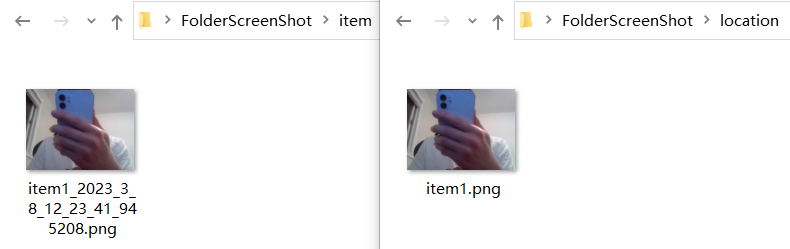
\includegraphics[width=90mm, height=35mm]{UT2.png}\\
  \hline
  Conclusion & Pass as expected\\
  \hline
\end{tabular}
\end{center}       
\caption{IPR5-1}
\end{table}
\newpage
\paragraph{Automatic Testing}{Testing shown:}

\begin{table}[H]
\begin{center}
\begin{tabular}{|l | m{9cm}|}
\hline
  Test Number & IPR6-1\\
  \hline
  Requirement Reference & IPR6\\
  \hline
  Requirement & The system should only make any update inside the location folder\\
  \hline
  Input & Start running the fileStorage function with the parameter, 'u', as updating\\
  \hline
  Desired Output & Only item1 get updated\\
  \hline
  Actual Output & Only item1.png get updated\\&Comparison shown:\\&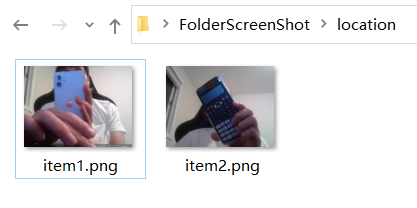
\includegraphics[width=90mm, height=46mm]{UT41.png}\\&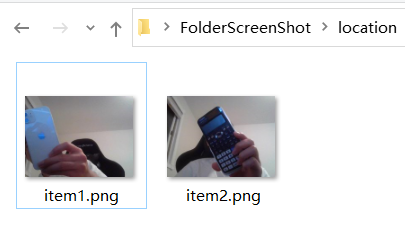
\includegraphics[width=89mm, height=48mm]{UT42.png}\\
  \hline
  Conclusion & Pass as expected\\
  \hline
\end{tabular}
\end{center}       
\caption{IPR6-1}
\end{table}

\begin{table}[H]
\begin{center}
\begin{tabular}{|l | m{9cm}|}
\hline
  Test Number & IPR7-1\\
  \hline
  Requirement Reference & IPR7\\
  \hline
  Requirement & The object information in the file folder should have unique IDs\\
  \hline
  Input & The automatic testing tool will call the file storage module and send the object information to the module\\
  \hline
  Desired Output & The different objects information will be stored in the folder with unique ID\\
  \hline
  Actual Output & The different objects information are stored in the folder with unique ID\\
  \hline
  Conclusion & Pass as expected\\
  \hline
\end{tabular}
\end{center}       
\caption{IPR7-1}
\end{table}

\begin{table}[H]
\begin{center}
\begin{tabular}{|l | m{9cm}|}
\hline
  Test Number & IPR8-1\\
  \hline
  Requirement Reference & IPR8\\
  \hline
  Requirement & The photos in the file folder should be sorted\\
  \hline
  Input & The automatic testing tool will call the photo storage function and send the photo to the module\\
  \hline
  Desired Output & The photos in the data storage module should be in ascending order of time\\
  \hline
  Actual Output & The photos in the data storage module are in ascending order of time\\
  \hline
  Conclusion & Pass as expected\\
  \hline
\end{tabular}
\end{center}       
\caption{IPR8-1}
\end{table}

\begin{table}[H]
\begin{center}
\begin{tabular}{|l | m{9cm}|}
\hline
  Test Number & IPR9-1\\
  \hline
  Requirement Reference & IPR9\\
  \hline
  Requirement & The photos in the file folder should be sorted\\
  \hline
  Input & The automatic testing tool will call the photo storage function and send the photo to the module\\
  \hline
  Desired Output & The photos in the data storage module should be in ascending or descending order of objects IDs\\
  \hline
  Actual Output & The photos in the data storage module are in ascending or descending order of objects IDs\\
  \hline
  Conclusion & Pass as expected\\
  \hline
\end{tabular}
\end{center}       
\caption{IPR9-1}
\end{table}

\subsubsection{UI Interface Menu}
\paragraph{Manual Testing}{Testing shown:}

\begin{table}[H]
\begin{center}
\begin{tabular}{|l | m{9cm}|}
\hline
  Test Number & UIR1-1\\
  \hline
  Requirement Reference & UIR1\\
  \hline
  Requirement & The UI should notify the user when the user highlights certain item\\
  \hline
  Input & User's manipulation to the user interface\\
  \hline
  Desired Output & The graphical displays to the user\\
  \hline
  Actual Output & 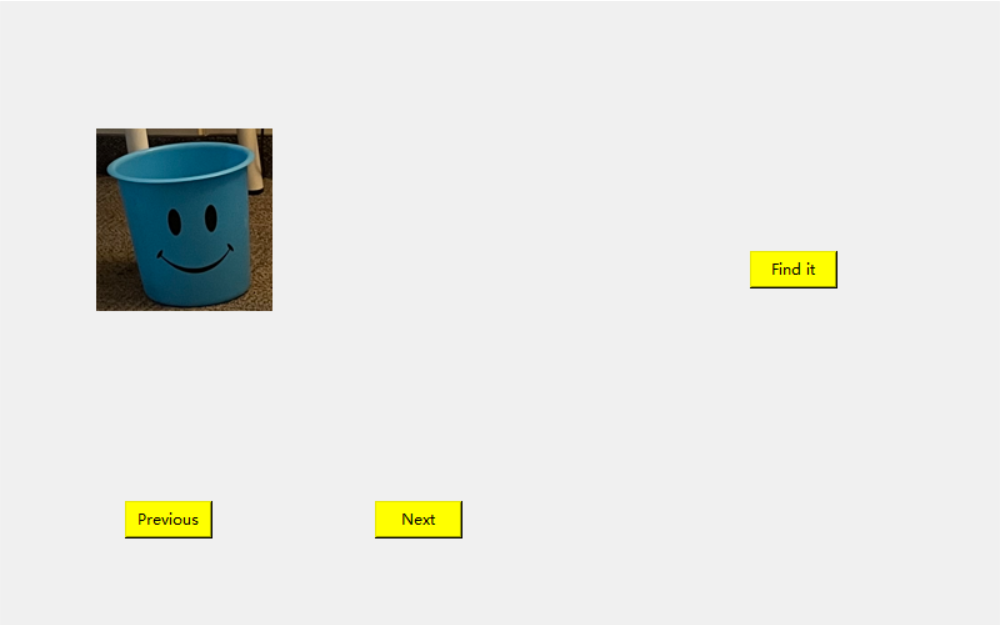
\includegraphics[width=80mm, height=55mm]{11.png}\\
  \hline
  Conclusion & The test is successful\\
  \hline
\end{tabular}
\end{center}    
\caption{UIR1-1}
\end{table}

\begin{table}[H]
\begin{center}
\begin{tabular}{|l | m{9cm}|}
\hline
  Test Number & UIR2-1\\
  \hline
  Requirement Reference & UIR2\\
  \hline
  Requirement & The UI should be able to let the user to change the sorting method\\
  \hline
  Input & User chooses another sorting method\\
  \hline
  Desired Output & The change between ascending and descending order\\
  \hline
  Actual Output & The change between ascending and descending order\\
  \hline
  Conclusion & The test is successful\\
  \hline
\end{tabular}
\end{center}   
\caption{UIR2-1}
\end{table}

\begin{table}[H]
\begin{center}
\begin{tabular}{|l | m{9cm}|}
\hline
  Test Number & UIR3-1\\
  \hline
  Requirement Reference & UIR3\\
  \hline
  Requirement & The UI should let the user have an access to the main menu\\
  \hline
  Input & The correct input of the password\\
  \hline
  Desired Output & Show the main menu in the UI window\\
  \hline
  Actual Output & Show the main menu in the UI window\\
  \hline
  Conclusion & The test is successful\\
  \hline
\end{tabular}
\end{center}   
\caption{UIR3-1}
\end{table}

\begin{table}[H]
\begin{center}
\begin{tabular}{|l | m{9cm}|}
\hline
  Test Number & UIR3-2\\
  \hline
  Requirement Reference & UIR3\\
  \hline
  Requirement & The UI should notify the user when the user has a wrong password input \\
  \hline
  Input & The wrong input of the password\\
  \hline
  Desired Output & There should be a text notification shown on the window\\
  \hline
  Actual Output & 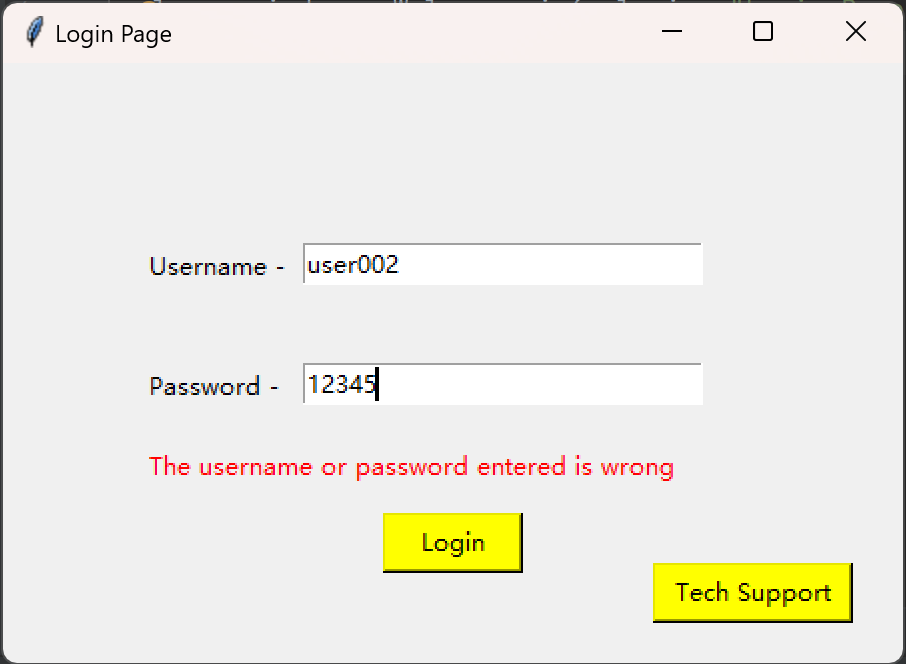
\includegraphics[width=80mm, height=55mm]{UIR11.png}\\
  \hline
  Conclusion & The test is successful\\
  \hline
\end{tabular}
\end{center}   
\caption{UIR3-2}
\end{table}



\begin{table}[H]
\begin{center}
\begin{tabular}{|l | m{9cm}|}
\hline
  Test Number & UIR4-1\\
  \hline
  Requirement Reference & UIR4\\
  \hline
  Requirement & The system should give the response on status identifier\\
  \hline
  Input & User changes and unplugs the camera to insert a fault\\
  \hline
  Desired Output & The graphical displays to the user\\
  \hline
  Actual Output & The application cannot be allowed to run since the camera is unplugged.\\
  \hline
  Conclusion & The test is successful\\
  \hline
\end{tabular}
\end{center}   
\caption{UIR4-1}
\end{table}

\begin{table}[H]
\begin{center}
\begin{tabular}{|l | m{9cm}|}
\hline
  Test Number & UIR5-1\\
  \hline
  Requirement Reference & UIR5\\
  \hline
  Requirement & The UI should be able to provide  technical support to the user\\
  \hline
  Input & The user press the technical support button\\
  \hline
  Desired Output & The technical support window is shown\\
  \hline
  Actual Output & 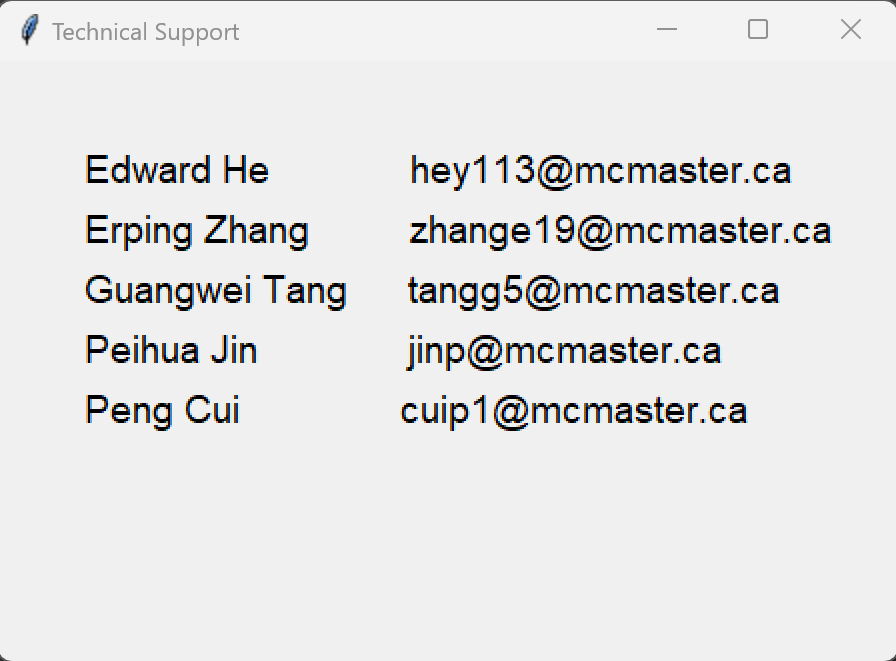
\includegraphics[width=80mm, height=55mm]{UIR51.png}\\
  \hline
  Conclusion & The test is successful\\
  \hline
\end{tabular}
\end{center}   
\caption{UIR5-1}
\end{table}

\section{Nonfunctional Requirements Evaluation}

\subsection{Usability}

\begin{table}[H]
\begin{center}
\begin{tabular}{|l | m{9cm}|}
\hline
  Test Number & APR1-1\\
  \hline
  Requirement Reference & APR1\\
  \hline
  Requirement & The User is able to launch the program without help\\
  \hline
  Input & The survey paper\\
  \hline
  Desired Output & An average of high rating shown on the paper\\
  \hline
  Actual Output & An average of 9.3 points on the rating of the usability of the program\\
  \hline
  Conclusion & The test is successful\\
  \hline
\end{tabular}
\end{center}   
\caption{APR1-1}
\end{table}

\begin{table}[H]
\begin{center}
\begin{tabular}{|l | m{9cm}|}
\hline
  Test Number & EUR1-1\\
  \hline
  Requirement Reference & EUR1\\
  \hline
  Requirement &  Users without electronics and coding background will be able to connect the hardware and use the program\\
  \hline
  Input & Users are asked to connect the hardware and start the program\\
  \hline
  Desired Output & There should not be any unclear instructions for the user to proceed. The hardware system including the Arduino board, camera and mount should be clarified for people to plug the wires\\
  \hline
  Actual Output & As camera,Arduino board and the motor are already attached to the mount. User just need to plug the wires to corresponding pins then they can simply start the program with one click \\
  \hline
  Conclusion & The test is successful\\
  \hline
\end{tabular}
\end{center}  
\caption{EUR1-1}
\end{table}

\begin{table}[H]
\begin{center}
\begin{tabular}{|l | m{9cm}|}
\hline
  Test Number & EUR2-1\\
  \hline
  Requirement Reference & EUR2\\
  \hline
  Requirement & The User is able to find the desired item without help\\
  \hline
  Input & The survey paper\\
  \hline
  Desired Output & An average of high rating shown on the paper\\
  \hline
  Actual Output & An average of 9.1 points on the usability of finding the item\\
  \hline
  Conclusion & The test is successful\\
  \hline
\end{tabular}
\end{center}     
\caption{EUR2-1}
\end{table}
\subsection{Performance}

\begin{table}[H]
\begin{center}
\begin{tabular}{|l | m{9cm}|}
\hline
  Test Number & SLR1-1\\
  \hline
  Requirement Reference & SLR1\\
  \hline
  Requirement & The User is able to find the desired item within certain time constraint\\
  \hline
  Input & Information of the object is entered properly\\
  \hline
  Desired Output & The response time of the system to show the location of the object should be less than 5 second\\
  \hline
  Actual Output & The average seconds is below 5 seconds\\
  \hline
  Conclusion & The test is successful\\
  \hline
\end{tabular}
\end{center}     
\caption{SLR1-1}
\end{table}

\begin{table}[H]
\begin{center}
\begin{tabular}{|l | m{9cm}|}
\hline
  Test Number & SCR3-1\\
  \hline
  Requirement Reference & SCR3\\
  \hline
  Requirement &  Rotation speed of the camera should be appropriate and will not damage other parts under the condition the camera have to rotate from one end to the other\\
  \hline
  Input & Human walk through the camera and leave the capture region at high pace\\
  \hline
  Desired Output & The camera will detect the human body and starts to follow the human movement. Once the human accelerate and leave the region, the camera will stop tracking and the rotation speed will not be fast enough to damage other parts\\
  \hline
  Actual Output & The camera will rotate to the human position and follow the movement once it detects the existence of human body. As the human quickly leave the capture region, the camera stops tracking and take a photo of the current frame. After 5 seconds, it will rotate back to the original position. There are no parts being damaged during the movement. And the angular velocity is under 30 degree/seconds \\
  \hline
  Conclusion & The test pass as expected\\
  \hline
\end{tabular}
\end{center}   
\caption{SCR3-1}
\end{table}

\begin{table}[H]
\begin{center}
\begin{tabular}{|l | m{9cm}|}
\hline
  Test Number & PAR2-1\\
  \hline
  Requirement Reference & PAR2\\
  \hline
  Requirement & The location value displayed should always be whole number\\
  \hline
  Input & The target object will be moved one small step at a time\\
  \hline
  Desired Output & The location value displayed should always be whole number\\
  \hline
  Actual Output & The displayed value is a whole number\\
  \hline
  Conclusion & The test is successful\\
  \hline
\end{tabular}
\end{center}     
\caption{PAR2-1}
\end{table}

\begin{table}[H]
\begin{center}
\begin{tabular}{|l | m{9cm}|}
\hline
  Test Number & RAR1-1\\
  \hline
  Requirement Reference & RAR1\\
  \hline
  Requirement & The user's work space is limited by certain angles\\
  \hline
  Input & The camera will keep rotating\\
  \hline
  Desired Output & The camera would never exceed the range of -180 degrees and +180 degrees\\
  \hline
  Actual Output & The motor stops at 180 degrees even if the human is still moving in a certain direction.\\
  \hline
  Conclusion & The test is successful\\
  \hline
\end{tabular}
\end{center}     
\caption{RAR1-1}
\end{table}

\begin{table}[H]
\begin{center}
\begin{tabular}{|l | m{9cm}|}
\hline
  Test Number & RFR2-1\\
  \hline
  Requirement Reference & RFR2\\
  \hline
  Requirement & The user is required to give appropriate instruction\\
  \hline
  Input & Wrong parameters will be entered into input boxes\\
  \hline
  Desired Output & The program will return error messages\\
  \hline
  Actual Output & Errors detected\\
  \hline
  Conclusion & The test is successful\\
  \hline
\end{tabular}
\end{center}     
\caption{RFR2-1}
\end{table}

\section{Demonstration Testing Requirement}
This section is aimed to test the stability and basic functionality for Revision-0 Demonstration.
\begin{table}[H]
\begin{center}
\begin{tabular}{|l | m{9cm}|}
\hline
  Test Number & DTR1\\
  \hline
  Requirement Reference & IPR5\\
  \hline
  Requirement &  To store the initial frame\\
  \hline
  Input & (1, 'i')\\
  \hline
  Desired Output & Adding item1\_\{date and time\}.png,  item1.png\\
  \hline
  Actual Output & Added as:\\&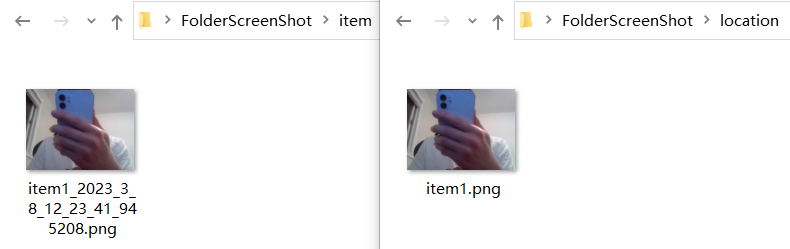
\includegraphics[width=90mm, height=35mm]{UT2.png}\\
  \hline
  Conclusion & Pass\\
  \hline
\end{tabular}
\end{center}    
\caption{DTR1}
\end{table}
\begin{table}[H]
\begin{center}
\begin{tabular}{|l | m{9cm}|}
\hline
  Test Number & DTR2\\
  \hline
  Requirement Reference & IPR5, IPR7\\
  \hline
  Requirement &  To check whether the frame is stored in the correct path\\
  \hline
  Input & (1, 'i')\\
  \hline
  Desired Output &  item\{num\}\_\{date and time\}.png is stored in 'item', item\{num\}.png is stored in 'location'\\
  \hline
  Actual Output &  item1\_2023\_3\_8\_12\_23\_41\_945208.png is within 'item', item1.png is inside 'location'\\&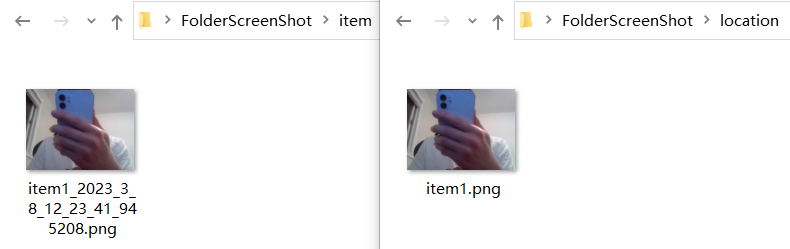
\includegraphics[width=90mm, height=35mm]{UT2.png}\\
  \hline
  Conclusion & Pass\\
  \hline
\end{tabular}
\end{center}  
\caption{DTR2}
\end{table}

\begin{table}[H]
\begin{center}
\begin{tabular}{|l | m{9cm}|}
\hline
  Test Number & DTR3\\
  \hline
  Requirement Reference & N/A\\
  \hline
  Requirement &  To create 3 folders sequentially\\
  \hline
  Input & createFolder() being called\\
  \hline
  Desired Output & 3 folders (FolderScreenShot, item, location) created\\
  \hline
  Actual Output & 3 folders (FolderScreenShot, item, location) created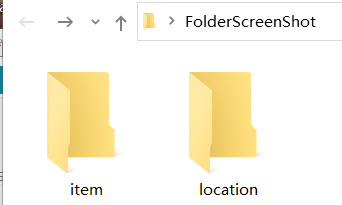
\includegraphics[width=80mm, height=55mm]{UT1.png}\\
  \hline
  Conclusion & Pass\\
  \hline
\end{tabular}
\end{center}   
\caption{DTR3}
\end{table}
\begin{table}[H]
\begin{center}
\begin{tabular}{|l | m{9cm}|}
\hline
  Test Number & DTR4\\
  \hline
  Requirement Reference & N/A\\
  \hline
  Requirement &  Do nothing if they have already existed\\
  \hline
  Input & createFolder() being called\\
  \hline
  Desired Output & No change\\
  \hline
  Actual Output & No change\\
  \hline
  Conclusion & Pass\\
  \hline
\end{tabular}
\end{center}    
\caption{DTR4}
\end{table}
\begin{table}[H]
\begin{center}
\begin{tabular}{|l | m{9cm}|}
\hline
  Test Number & DTR5\\
  \hline
  Requirement Reference & IPR5, IPR6\\
  \hline
  Requirement & To check whether the frame for the second item is captured\\
  \hline
  Input & (2, 'i')\\
  \hline
  Desired Output & Adding item2\_\{date and time\}.png, item2.png\\
  \hline
  Actual Output & Added as:\\&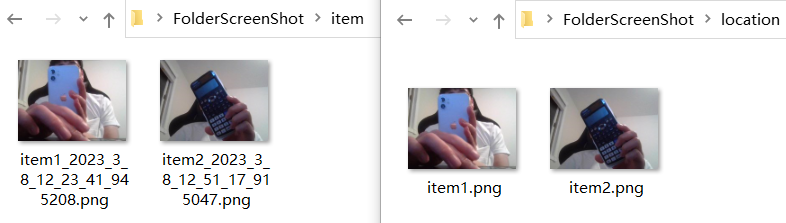
\includegraphics[width=90mm, height=33mm]{UT3.png}\\
  \hline
  Conclusion & Pass\\
  \hline
\end{tabular}
\end{center}   
\caption{DTR5}
\end{table}
\begin{table}[H]
\begin{center}
\begin{tabular}{|l | m{9cm}|}
\hline
  Test Number & DTR6\\
  \hline
  Requirement Reference & IPR4, IPR6\\
  \hline
  Requirement &  To check whether the location frame for the first item is updated, meanwhile the second item won't get affected\\
  \hline
  Input & (1, 'u')\\
  \hline
  Desired Output & item1\_\{date and time\}.png should remain, item1.png shall be updated\\
  \hline
  Actual Output & Only item1.png get updated\\&Comparison shown:\\&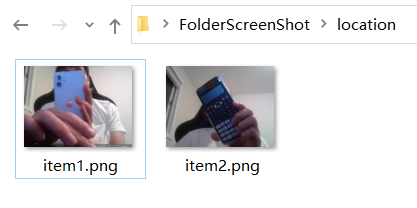
\includegraphics[width=90mm, height=46mm]{UT41.png}\\&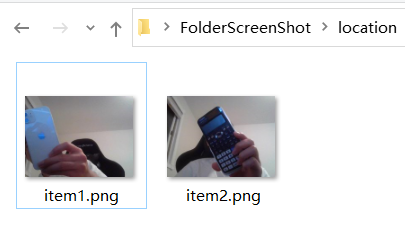
\includegraphics[width=89mm, height=48mm]{UT42.png}\\
  \hline
  Conclusion & Pass\\
  \hline
\end{tabular}
\end{center} 
\caption{DTR6}
\end{table}

\section{Changes Due to Testing}
Based on the feedback from Rev 0 demo, we have conducted our test case based on larger room with more complex background environments. During the early stages of testing process, performance reliability issues were found, which led to changes to the main algorithm which aims to lower the light sensitivity to increase the repeatability of the test cases.  \\
 
 Taking notes from our discussion with users, we tried to best limit the user interaction with the system. Users is only required to interact with the user interface which has adapted to user feedback to improve usability. \\
 
 Another point noted was that users would like to have more detailed time for searching specific items. This will be implemented in the upcoming milestone where some other quality of life update will be implemented. \\

\section{Traceability Matrices}
\subsection{Traceability for Image Processing and Functional Requirements}
\begin{table}[H]
\begin{tabular}{|p{0.33\textwidth}|p{0.33\textwidth}|p{0.33\textwidth}|}

\hline Test Method&Requirement&Test Number\\

\hline Manual&IPR1&IPR1-1\\

\hline Manual&IPR1&IPR1-2\\

\hline Manual&IPR1&IPR1-3\\

\hline Manual&IPR2&IPR2-1\\

\hline Manual&IPR2&IPR2-2\\

\hline Manual&IPR2&IPR2-3\\

\hline Manual&IPR3&IPR3-1\\

\hline Manual&IPR4&IPR4-1\\

\hline Manual&IPR5&IPR5-1\\

\hline Automatic&IPR6&IPR6-1\\

\hline Automatic&IPR7&IPR7-1\\

\hline Automatic&IPR8&IPR8-1\\

\hline Automatic&IPR9&IPR9-1\\

\hline

\end{tabular}
\caption{Traceability for Image Processing and File Storage Testing}
\end{table}
\\
\begin{table}[H]
\begin{tabular}{|p{0.33\textwidth}|p{0.33\textwidth}|p{0.33\textwidth}|}

\hline Test Method&Requirement&Test Number\\

\hline Manual&UIR1&UIR1-1\\

\hline Manual&UIR2&UIR2-1\\

\hline Manual&UIR3&UIR3-1\\

\hline Manual&UIR3&UIR3-2\\

\hline Manual&UIR4&UIR4-1\\

\hline Manual&UIR5&UIR5-1\\

\hline

\end{tabular}
\caption{Traceability for UI Interface Menu}
\end{table}
\subsection{Traceability for Nonfunctional Requirements}

\begin{table}[H]
\begin{tabular}{|p{0.33\textwidth}|p{0.33\textwidth}|p{0.33\textwidth}|}

\hline Test Method&Requirement&Test Number\\

\hline Structural, Manual&APR1&APR1-1\\

\hline Functional, Manual&EUR1&EUR1-1\\

\hline Functional, Manual&EUR2&EUR2-1\\

\hline Functional, Manual&SLR1&SLR1-1\\

\hline Functional, Manual&SCR3&SCR3-1\\

\hline Functional, Manual&PAR2&PAR2-1\\

\hline Functional, Manual&RAR1&RAR1-1\\

\hline Functional, Manual&RFR2&RFR2-1\\

\hline

\end{tabular}
\caption{Traceability for Usability and Humanity Requirements}
\end{table}

\subsection{Traceability for Demonstration Testing Requirements}
\begin{table}[H]
\begin{tabular}{|p{0.33\textwidth}|p{0.33\textwidth}|p{0.33\textwidth}|}

\hline Test Method&Requirement&Test Number\\
\hline Manual&IPR5&DTR1\\
\hline Manual&IPR5, IPR7&DTR2\\
\hline Manual&N/A&DTR3\\
\hline Manual&N/A&DTR4\\
\hline Manual&IPR5, IPR6&DTR5\\
\hline Manual&IPR4, IPR6&DTR6\\
\hline

\end{tabular}
\caption{Traceability for Image Processing and File Storage Testing}
\end{table}

\bibliographystyle{plainnat}
\bibliography{../../refs/References}

\newpage{}
\section*{Appendix --- Reflection}

The information in this section will be used to evaluate the team members on the
graduate attribute of Lifelong Learning.  Please answer the following questions:


\begin{enumerate}
  \item In what ways was the Verification and Validation (VnV) Plan different
  from the activities that were actually conducted for VnV?  If there were
  differences, what changes required the modification in the plan?  Why did
  these changes occur?  Would you be able to anticipate these changes in future
  projects?  If there weren't any differences, how was your team able to clearly
  predict a feasible amount of effort and the right tasks needed to build the
  evidence that demonstrates the required quality?  (It is expected that most
  teams will have had to deviate from their original VnV Plan.)
  
  
\end{enumerate}
 One of the biggest area of difference between VnV plan and VnV report is from some of the changes to the functional requirements. Our system is no longer tracking human hands, which reflected in the VnV report where we did not test that specific requirement. Another difference is that we modified the logic of camera and motor movement. The purpose of this modification is to satisfy the image process requirement, which cause we add a new requirement and test case compare with the VnV plan. What's more, The test for opening the technical support window is added because the path for the customer to ask help from the program developer is important. Since VnV plan was made prior to us finalizing the implementation, we had made several assumptions that were later modified. However, most of our VnV plan turned out to be feasible and essential for the validation of our project. Since we developed our testing plan based on input/outcome, the change to our anticipated algorithm did not affect the general path for our VnV report. The proposed testing case in VnV plan were tested and validated.
 
 



\end{document}
